\chapter{Setup}

Dieses Kapitel behandelt die Installation und Ersteinrichtung der Suchmaschine. Die Installation erfolgt dabei über Docker mithilfe von Docker-Compose. Es werden 2 Elasticsearch-Instanzen, eine Kibana-Instanz und eine Logstash-Instanz aufgesetzt. Das fertig Setup soll dann wie folgt aussehen \ref{img:dockerNetwork}.

\begin{figure}
	\centering
	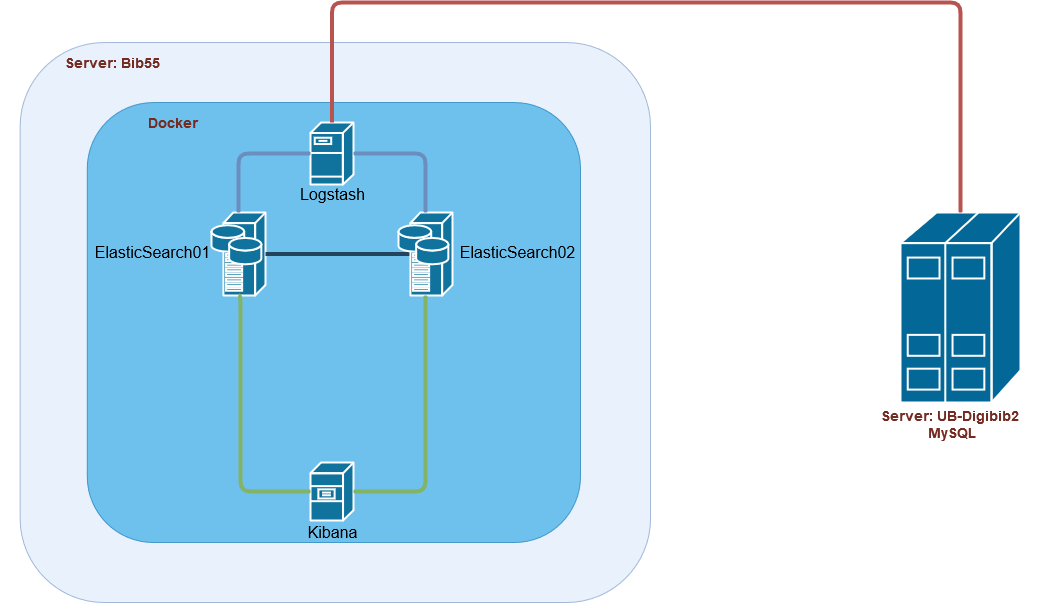
\includegraphics[width=1\linewidth]{images/docker_structure.png}
	\caption{Visualisierung des fertiges Docker-Netzwerkes}
	\label{img:dockerNetwork}
\end{figure}

Logstash sammelt die Daten von einem MySQL-Server und lädt sie in die Elasticsearch-Instanzen. Auch Kibana bekommt Zugriff auf beide Instanzen, um die Daten zu visualisieren und bei Serverausfällen frühzeitig zu warnen. Die beiden Elasticsearch-Instanzen halten sich dabei untereinander synchron. 

\section{Docker}

Docker ist eine Software zur Virtualisierung von Anwendungen. Dabei wird allerdings nicht, wie bei virtuellen Maschinen, die gesamte Hardware simuliert, sondern sie laufen im Kontext des Host-Betriebstystems.

Docker-Compose ist ein Tool, mit welchem es erleichtert wird, mehrere Docker-Container zu verwalten. Dafür werden in einer YAML-Datei\footnote{Kurz für YAML Ain't Markup Language, eine Konfigurationssprache \url{https://yaml.org/}} die gewünschten Docker-Container und Einstellungen, wie der Container-Name, eingetragen \ref{lst:es01}. Mithilfe dieser Datei erstellt Docker-Compose dann die Container und Netzwerke automatisch.

\subsection{Rechteverwaltung in Docker}

Ein kurzer Exkurs zur Rechteverwaltung in Docker. Will ein Docker-Container auf dem Host-System schreiben, so nutzt dieser die Berechtigungen des Users innerhalb des Docker-Containers. Es kann allerdings passieren, dass die Nutzer-ID des Docker-Containers nicht der Nutzer-ID des Hosts entspricht. Werden nun Dateien im Hostsystem abgelegt, welche vom Container gelesen werden, muss dabei auf die Rechte geachtet werden. 

Elasticsearch verwendet die UID\footnote{Kurz für User identifier, Zahl zur Bestimmung eines Nutzers} und GID\footnote{Kurz für Group identifier, Zahl zur Bestimmung einer Nutzergruppe} von 1000. Auf dem Host-System ist dies jedoch ein anderer Nutzer. Das kann zu Problemen führen, da nun Dateien, welche für Elasticsearch gedacht sind, einem Nutzer, welcher nicht zu diesem Projekt gehört, gehören. Der Nutzer wurde nun auf eine andere UID gesetzt, um Verwirrung zu vermeiden. \cite{JarrodWeaver.2014}

\section{Elasticsearch}

Die beiden Elasticsearch-Instanzen bilden das Kernstück dieses Setups. Sie werden die Daten verwalten und sich untereinander synchronisieren. Dafür werden die beiden Instanzen als Cluster betrieben.

\begin{lstlisting}[language=YAML, frame=single, label={lst:es01}, caption=Auschnitt aus der Docker-Compose Datei,captionpos=b] 
es01:
image: docker.elastic.co/elasticsearch/elasticsearch:7.5.1
container_name: es01
environment:
	- "ES_JAVA_OPTS=-Xms4g -Xmx4g"
ulimits:
	memlock: -1
volumes:
	- /srv/elk/elasticSearch01/:/usr/share/elasticsearch/data
	- /srv/elk/config/elasticsearch.yml:
		/usr/share/elasticsearch/config/elasticsearch.yml
ports:
	- 9200:9200
networks:
	- elastic
\end{lstlisting}

Das Listing \ref{lst:es01} zeigt einen Auschnitt aus der Docker-Compose, in welchem die ersten Einstellungen getroffen werden.

Für die beiden Elasticsearch-Instanzen wird der Java-Speicher auf 4 Gigabyte gesetzt. Dies errechnet sich dadurch, dass der Server 16 Gigabyte RAM besitzt und die Elasticsearch-Instanzen nicht mehr als 50 \% des gesamten RAMs verwenden sollten. \cite{ElasticsearchB.V..12172019}

Der ulimits Befehl hebt die Begrenzung des Memory-Locks auf, damit Elasticsearch korrekt arbeiten kann. Dadurch wird der RAM von Elasticsearch nicht in den SWAP-Speicher\footnote{Speicher auf der Festplatte, welcher von Linux genutzt wird, falls der RAM voll ist.} gelegt. Dies würde die Leistung von der Suchmaschine stark beinträchtigen.

Als Volumes ist zum einen die oben genannte YAML-Datei angegeben und zum anderen wird der Datenordner gemountet. Dies dient dazu, dass, falls der Container zerstört wird, die indexierten Daten trotzdem weiterhin auf dem Host-System verbleiben.

Der Port wird zum Host-System durchgereicht, damit das System auch von außerhalb des Docker-Netwerkes zu erreichen ist. Dabei ist das System trotz blockierter UFW\footnote{UFW ist die uncomplicated Firewall, eine Firewall-Software für Linux} zu erreichen. Dies liegt daran, dass die Docker-Container in der Standardeinstellung die UFW ignorieren.

In der Elasticsearch-Konfigurationsdatei werden nun die Einstellungen, die speziell für das Elasticsearch-System relevant sind, verwaltet: 

\begin{lstlisting}[language=YAML, frame=single, label={lst:es01-yml}, caption=Auschnitt aus der Konfigurationsdatei von Elasticsearch,captionpos=b] 
cluster.name: dietrich-online-cluster
node.name: es01
bootstrap.memory_lock: true
network.host: 0.0.0.0
discovery.seed_hosts: ["es02"]
cluster.initial_master_nodes: ["es01", "es02"]
\end{lstlisting}

Darin wird zuerst der Cluster-Name definiert. Dieser dient dazu, dass die Server wissen, dass sie dieselben Daten betreuen. 
Danach wird der Name des Servers vergeben, welcher der Identifizierung dient.

Das Memory-Lock Setting dient dazu, dass die Anwendung verhindert, dass sie in den SWAP gelegt wird.

Der Network Host wird hier auf alle Interfaces der Maschine gesetzt, damit sich alle Systeme innerhalb der Docker-Netzwerkes finden können.

Das Seed-Host Setting sagt aus, an welchen Nodes\footnote{Hier: Elasticsearch-Instanzen} die Daten synchronisiert werden sollen.

Der letzte Eintrag dient dazu, dass bei der ersten Synchronisation das System weiß, welche Nodes alle Daten enthalten, also mit welchen Server sich synchronisiert werden soll. Da hier beide Systeme beim ersten Start noch keine Daten besitzen, sind alle Nodes zu beginnt Master. 


\section{Kibana}

Die Grundkonfiguration von Kibana ist einfacher als die Konfiguration von Elasticsearch. Es muss nur die YAML-Datei in den Container geladen werden und der Port 5601 nach außen durchgereicht werden.

In der Konfigurationsdatei werden nun die Einstellungen für Kibana gesetzt. Darunter fällt der oben genannte Port, der Server-Host, in diesem Fall auch 0.0.0.0, und die Elasticsearch-Hosts. Dabei werden alle Server-Instanzen mitgegeben, auf denen Kibana arbeiten soll. 

\section{Logstash}

Für die Grundkonfiguration von Logstash muss, wie schon im Ersteindruck, der Treiber in die Core-Bibliothek gelegt werden. Zudem werden die Konfigurationsdateien für die Pipelines gemountet.

In der Konfigurationsdatei für Logstash wird dann der Name, die Pipeline.id und die Pipeline-Worker festgelegt. Die Pipeline-Worker sind die Threads, in denen eine der konfigurierten Pipelines abgearbeitet wird. Generell sollte die Anzahl der Cores auch die maximale Anzahl der Worker sein.


\section{X-Security}

X-Security nennt sich das Paket, mit den Sicherheitseinstellungen für den ELK-Stack. In diesem Schritt wird der komplette Datenverkehr zwischen den einzelnen Komponenten, sowie vom Endnutzer zum Server mit SSL verschlüsselt. 

Dazu werden zuerst die Zertifikate generiert. Dafür bietet Elasticsearch ein Tool an, welches eine Zertifikats-Autorität (CA)\footnote{Mithilfe einer CA kann sich ein Klient gegenüber des Servers ausweisen und umgekehrt.} und die einzelnen Zertifikate mit Private- und Public-Key generiert. Allerdings werden diese standardmäßig im PKCS 12-Format abgespeichert. Dieses ist ein Container-Format, welches die Schlüssel und die CA zusammen verpackt. Jedoch benötigt Kibana zum Beispiel nur die Autorität als einzelnes Zertifikat und nicht den Container.

Normalerweise gibt es eine Möglichkeit, dieses Zertifikat aus der PK12-Datei zu entpacken, jedoch gab es hierbei Probleme, da OpenSSL, das Tool welches zum Entpacken verwendet wird, die CA nicht richtig entpacken kann. \cite{nerophon.2018}

Die Lösung dieses Problems war es, schon bei der Zertifikaterstellung eine Option mitzugeben, dass die Zertifikate nicht verpackt werden sollen. 

Um nun alle Zertifikate gleichzeitig zu generieren, kann eine YAML-Datei mitgegeben werden. In dieser werden dann die Details für die Zertifikate, wie zum Beispiel DNS-Name und IP des Servers, mitgegeben. In diesem Fall wurde nur der DNS-Name angegeben \ref{lst:certs-yml}:

\begin{lstlisting}[language=YAML, frame=single, label={lst:certs-yml}, caption=Auschnitt aus der Konfigurationsdatei für die Zertifikatgenerierung,captionpos=b] 
instances:
- name: 'es01'
	dns: [ 'es01', 'bib55', 'bib55.uni-trier.de' ]
[...]
\end{lstlisting}

Damit diese Zertifikate auch genutzt werden können, muss jeder Container das zugehörige Zertifikat einbinden. Zudem wurden in den dazugehörigen Konfigurationsdateien die jeweiligen Optionen zur Nutzung der CA und Private-Keys gesetzt.

Zusätzlich zu den Zertifikaten muss noch eine Passwort-Authentifikation eingebaut werden. Dazu kann auf den Elasticsearch-Containern ein Befehl zur Erstellung der Systempasswörter aufgerufen werden. Dadurch werden alle Benutzer, welche die einzelnen Systeme wie Logstash oder Kibana zum Funktionieren brauchen, generiert.

Auch diese müssen in den Konfigurationsdateien vermerkt werden. Weitere Nutzer können von nun an per API oder Kibana erstellt werden. Die Verteilung der Rechte ist hierbei rollenbasiert. Es wird zuerst eine Rolle erstellt, welche die gewünschten Rechte enthält, welche daraufhin an den Nutzer weitergegeben wird. Dabei können die Rollen sehr spezifisch angepasst werden. Es können einzelne Systemfunktionen, wie die Erstellung von Snapshots, spezifisch freigegeben werden. Hierbei sollte sich an das Minimalprinzip gehalten werden, also nur genau die Rechte vergeben werden, welche der Nutzer auch benötigt. Zusätzliche Rechte werden dem Nutzer dabei verwehrt.

Um nun eine Abfrage gegen das Elasticsearch-System zu stellen, muss zum einen eine BasicAuth, sowie die CA mitgegeben werden:

\begin{lstlisting}[language=BASH, frame=single, label={lst:curlQuery}, caption=Curl-Abfrage an das Elasticsearch-System,captionpos=b] 
curl https://bib55:9200 --cacert ca.crt -uuser:pass
\end{lstlisting}

Damit Logstash wieder Daten an Elasticsearch senden kann, wird ein Nutzer erstellt, welcher nur auf Indices mit dem Präfix dietrich\_ Zugriff erhält. Die Erstellung von diesem Nutzer erfolgte dabei über die Benutzer-Oberfläche von Kibana \ref{img:kibanaRoles}. 

\begin{figure}
	\centering
	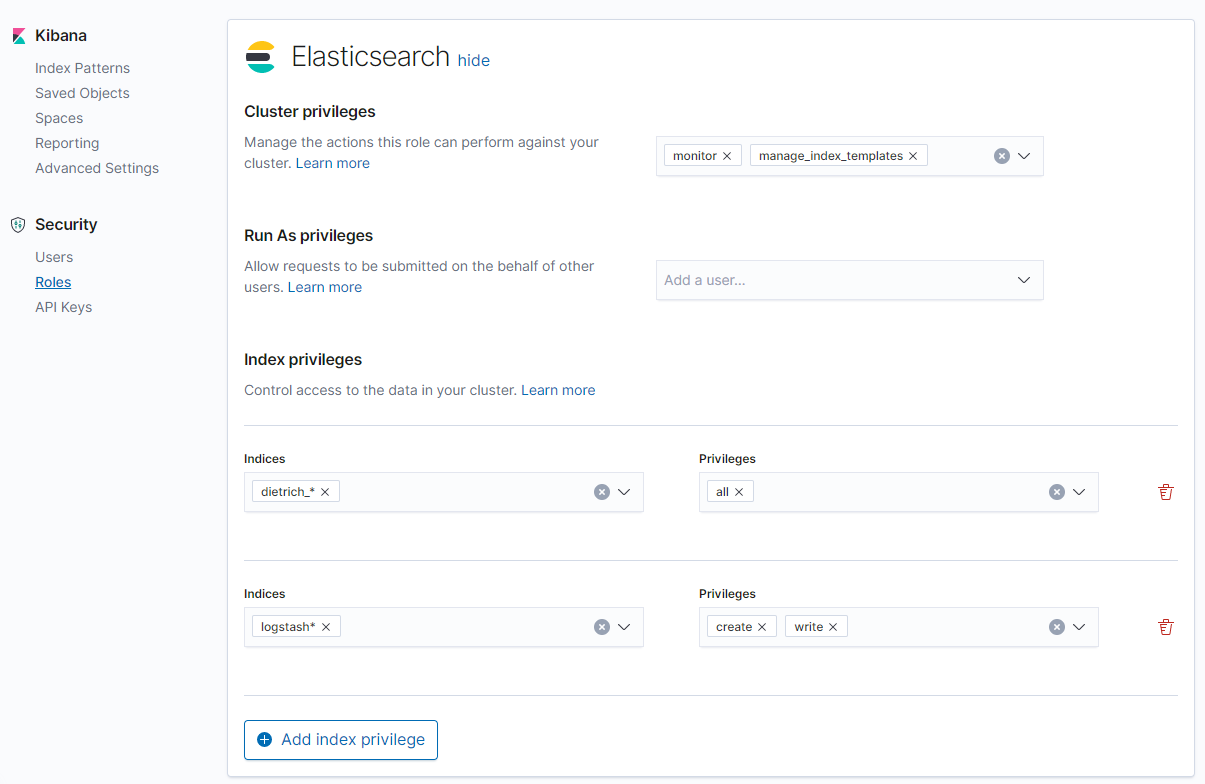
\includegraphics[width=1\linewidth]{images/setup/kibana_roles.png}
	\caption{Seite zu Erstellung von Rechte-Rollen}
	\label{img:kibanaRoles}
\end{figure}